%\documentclass{jss}
\documentclass[nojss]{jss}
\usepackage[OT1]{fontenc}
%\usepackage[latin1]{inputenc}
\usepackage{graphicx}
\usepackage{amsmath}

%\usepackage{cite}
\usepackage{draftwatermark}
\SetWatermarkText{Draft}
\SetWatermarkScale{1.5}

%\usepackage{myVignette}

%\VignetteIndexEntry{The MBBEFD package}
%\VignetteKeywords{vig1}
%\VignettePackage{mbbefd}
% need no \usepackage{Sweave.sty}

%\SweaveOpts{prefix.string=Figures/fig}
%%%%%%%%%%%%%%%%%%%%%%%%%%%%%%
%% declarations for jss.cls %%%%%%%%%%%%%%%%%%%%%%%%%%%%%%%%%%%%%%%%%%
%%%%%%%%%%%%%%%%%%%%%%%%%%%%%%

%% almost as usual
\author{Giorgio Alfredo Spedicato, Ph.D C.Stat ACAS}
\title{The \pkg{mbbefd} Package: A Package for handling MBBEFD exposure curves in \proglang{R}}

%% for pretty printing and a nice hypersummary also set:
\Plainauthor{Giorgio Alfredo Spedicato, Ph.D C.Stat ACAS} %% comma-separated
\Plaintitle{The mbbefd Package: A Package for handling MBBEFD exposure curves in R} %% without formatting
\Shorttitle{The mbbefd package} %% a short title (if necessary)
%% an abstract and keywords
\Abstract{The package models MBBEFD distribution providing density, quantile, distribution and random generation functions. In addition it provides exposure curves for the MBBEFD distribution family.
}
\Keywords{mbbefd, exposure curves, reinsurance, non-life insurance}
\Plainkeywords{mbbefd, exposure curves, reinsurance, non-life insurance} %% without formatting
%% at least one keyword must be supplied

%% publication information
%% NOTE: Typically, this can be left commented and will be filled out by the technical editor
%% \Volume{13}
%% \Issue{9}
%% \Month{September}
%% \Year{2004}
%% \Submitdate{2004-09-29}
%% \Acceptdate{2004-09-29}

%% The address of (at least) one author should be given
%% in the following format:
\Address{
  Giorgio Alfredo Spedicato\\
  StatisticalAdvisor\\
  Via Firenze 11
  20037 Italy\\
  Telephone: +39/334/6634384\\
  E-mail: \email{spedicato\_giorgio@yahoo.it}\\
  URL: \url{www.statisticaladvisor.com}
}


%% for those who use Sweave please include the following line (with % symbols):
%% need no \usepackage{Sweave.sty}

%% end of declarations %%%%%%%%%%%%%%%%%%%%%%%%%%%%%%%%%%%%%%%%%%%%%%%

\begin{document}


\maketitle


\section{Introduction}

The \pkg{mbbefd} package provides function to use Maxwell-Bolzano, Bose-Einstein, Fermi-Dirac probability distributions, introduced by \citep{bernegger1997tile}, within \proglang{R} statistical software \citep{rSoftware}.\\ Such kind of distributions are widely used in the pricing of non-life reinsurance contracts and yet they are not present in any R package.\\

The paper is structured as follows: Section~\ref{sec:review} discusses review the theory (mathematics and actuarial application) of MBBEFD distributions, Section~\ref{sec:package} shows the package's features, applied examples are shown in Section~\ref{sec:examples} while the issue of fitting MBBEFD curves to empirical data is discussed in Section~\ref{sec:fitting}.\\



\section{Exposure curve review}\label{sec:review}

Within actuarial jargon, an exposure curve is a distribution that shows the ratio between the expected limited loss at various limits and the expected unlimited loss. They are usually to rate large commercial risks' exposures and non-proportional reinsurance treaties. In mathematical notation, if $IV$ is the insured value and $d$ the ratio of loss $x$ to $IV$ the exposure curve $G\left( d \right)$ is defined as Equation~\ref{eq:expoCurve} displays.

\begin{equation}
G\left( d \right) = \frac{{E\left[ {\min \left( {d*IV,x} \right)} \right]}}{{E\left[ x \right]}} = \frac{{\int_0^{d*IV} {\left( {1 - F\left( x \right)} \right)dx} }}{{\int_0^\infty  {x*f\left( x \right)dx} }} = \frac{{\int_0^{d*IV} {S\left( x \right)dx} }}{{\int_0^\infty  {S\left( x \right)dx} }}
\label{eq:expoCurve}
\end{equation}

Whilst losses normally lie in the interval $0,\ldots, \infty$ for the rest of the paper it will be assumes $x$ to represent a normalized loss in the interval $0,\ldots, PML$, being $PML$ the so - called maximum probable loss (in other words, the maximum loss it is thought to can happen). Therefore $x$ would represent a percentage loss with respect to a maximum, i.e., a destruction rate.\\


\cite{bernegger1997tile} and \cite{mahler} provide a discussion on the actuarial theory regarding such curve. In particular, the curves discussed by \cite{bernegger1997tile} are of the form expressed by Equation~\ref{eq:expoCurve2}.

\begin{equation}
\left\{ \begin{array}{l}
G\left( x \right) = \frac{{\ln \left( {a + {b^x}} \right) - \ln \left( {a + 1} \right)}}{{\ln \left( {a + b} \right) - \ln \left( {a + 1} \right)}}\\
x \in \left[ {0,1} \right]
\end{array} \right.
\label{eq:expoCurve2}
\end{equation}

It can be shown that $G \left( 0 \right)=0$, $G\left( 1 \right)=1$, $dG \left( d \right) \ge 0$ and $ddG \left( d \right) \le 0$. Using some calculus on Equation~\ref{eq:expoCurve2} it can be shown that the expected value is equal to the reciprocal of exposure curve derivative at 0, Equation~\ref{eq:expectedValue}.\\

\begin{equation}
  \mu = \frac{1}{dG \left( 0 \right) }
  \label{eq:expectedValue}
\end{equation}

The probability of a total loss, $p$, is expressed by Equation~\ref{eq:totalLoss}.

\begin{equation}
p = 1 - F\left( 1^{-}  \right) = \frac{1}{g} = \frac{dG\left( 1 \right)}{dG\left( 0 \right)} = \frac{\left( a + 1 \right)*b}{a + b}
\label{eq:totalLoss}
\end{equation}

It is similarly possible to write expression for the Survival Function, $S \left( x \right)$, Equation~\ref{eq:survival} and the density, Equation~\ref{eq:density}.

\begin{equation}
S\left( x \right) = \frac{{G'\left( x \right)}}{{G'\left( 0 \right)}} = \frac{{\left( {a + 1} \right){b^x}}}{{a + {b^x}}}
\label{eq:survival}
\end{equation}

\section{The MBBEFD class and its related package}\label{sec:package}

\begin{Schunk}
\begin{Sinput}
R> library(mbbefd)
\end{Sinput}
\end{Schunk}


The \code{mbbefdExposure} function evaluates the exposure curve for a given destruction rate $x$, given either $a$ and $b$, or $b$ and $g$. Figure~\ref{fig:G1} displays the destruction rate by level of x, for an exposure cuve of parameters $a=0.2$ and $b=0.04$



\begin{figure}
\begin{center}
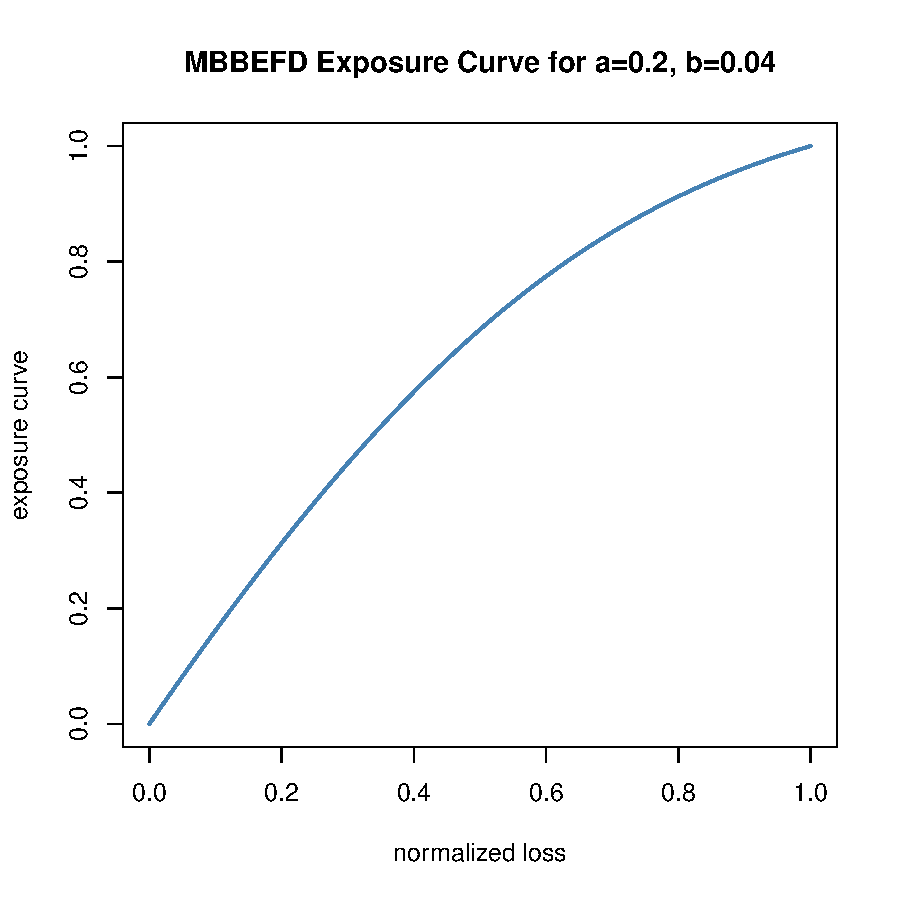
\includegraphics{mbbefd-drateplot}
\caption{Exposure curve example}
\label{fig:G1}
\end{center}
\end{figure}



\section{Applied examples}\label{sec:examples}
The curve can be use to price property coverage and associate reinsurance treaties. Suppose a property expected loss to be 40K, MPL to be 2MLN. An XL coverage is available with a retention of 1Mln. The exposure curve that characterize the property is the usual one. Therefore the percentage of loss net and ceded is determined as it follows

\begin{Schunk}
\begin{Sinput}
R> net<-mbbefdExposure(x=1/2, a=0.2,b=0.04)*40000
R> ceded<-40000-net
\end{Sinput}
\end{Schunk}

and the expected loss as a percentage of total insured value is

\begin{Schunk}
\begin{Sinput}
R> expectedLoss<-1/dG(x=0,a=0.2,b=0.04)*40000
R> expectedLoss
\end{Sinput}
\begin{Soutput}
[1] 24000
\end{Soutput}
\end{Schunk}


Similarly, it is possible to draw the underluying suvival curve $S\left( x \right) = \frac{{G'\left( x \right)}}{{G'\left( 0 \right)}}$ using  Figure~\ref{fig:survival}.

\begin{figure}
\begin{center}
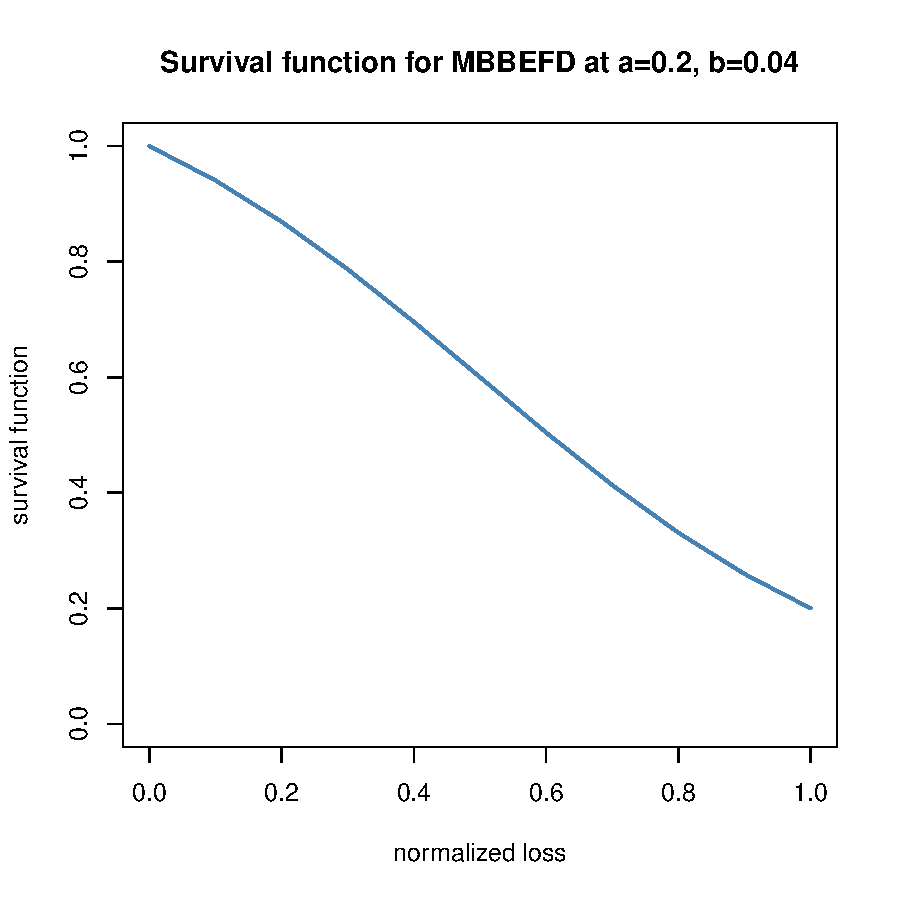
\includegraphics{mbbefd-survivalPlot}
\caption{Underlying survival curve}
\label{fig:survival}
\end{center}
\end{figure}


The probability of a maximum loss for such exposure curve is obtained evaluating the survival function at 1

\begin{Schunk}
\begin{Sinput}
R> pTotalLoss<-1-pmbbefd(q=1,a=0.2,b=0.04)
R> pTotalLoss
\end{Sinput}
\begin{Soutput}
[1] 0.2
\end{Soutput}
\end{Schunk}

Similarly, it is possible to assess the mean of the distribution underlying the exposure curve 


Quantile functions, distribution functions and density functions are defined as well. For example, the 60th percentile of the distribution above defined (i.e., how bad can be in 60\% of cases in terms of destruction rate) is

\begin{Schunk}
\begin{Sinput}
R> qmbbefd(p=0.6,a=0.2,b=0.04)
\end{Sinput}
\begin{Soutput}
[1] 0.7153383
\end{Soutput}
\end{Schunk}

whilst a loss worse than 80\% of IV could happen in 

\begin{Schunk}
\begin{Sinput}
R> 100*(1-pmbbefd(q=0.8,a=0.2,b=0.04))
\end{Sinput}
\begin{Soutput}
[1] 33.0895
\end{Soutput}
\end{Schunk}

cases out of 100.

It would be possible to simulate variates from the MBBEFD distribution using the 
random generation command \code{rmbbefd}.

\begin{Schunk}
\begin{Sinput}
R> simulatedLosses<-rmbbefd(n=10000,a=0.2,b=0.04)
R> mean(simulatedLosses)
\end{Sinput}
\begin{Soutput}
[1] 0.597828
\end{Soutput}
\begin{Sinput}
R> sum(simulatedLosses==1)/length(simulatedLosses)
\end{Sinput}
\begin{Soutput}
[1] 0.1949
\end{Soutput}
\end{Schunk}

\begin{figure}
\begin{center}
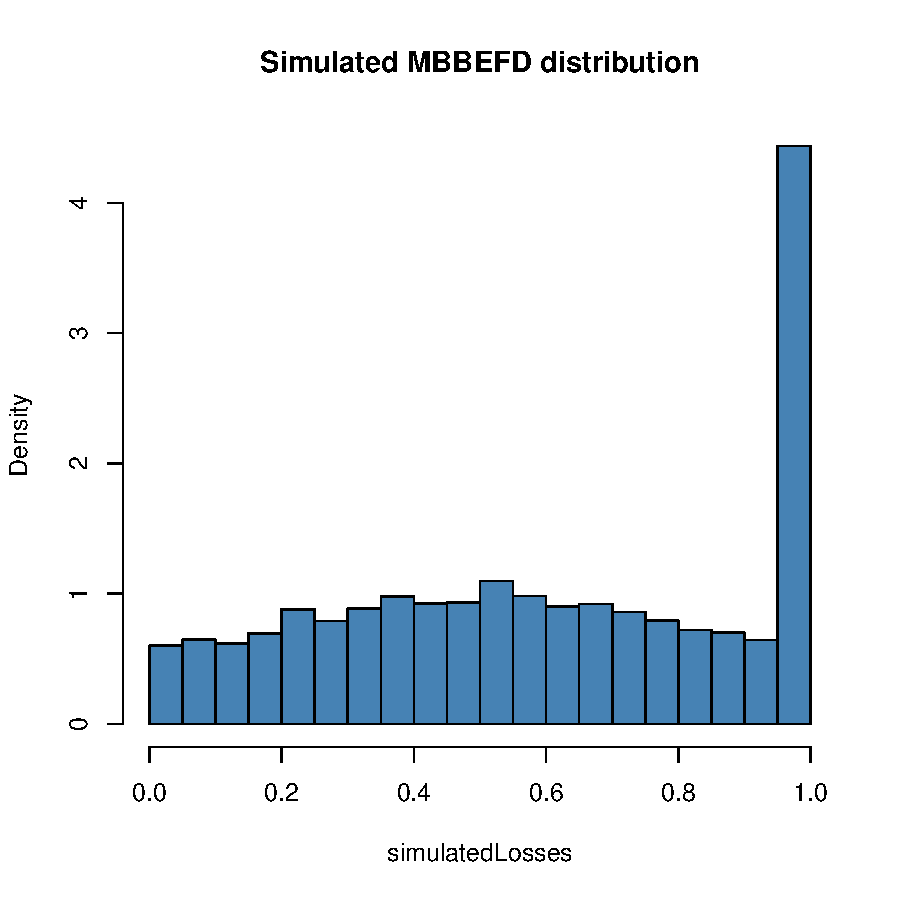
\includegraphics{mbbefd-distrPlot}
\caption{Exposure curve example}
\label{fig:G1}
\end{center}
\end{figure}




Finally another way to show the probability of total loss to be greater than zero is to show that the (numerical) integral between 0 and 1 of the density function is lower than 1, that is $1-F\left(1^- \right)$.

\begin{Schunk}
\begin{Sinput}
R> integrate(dmbbefd,lower=0, upper=1, a=0.2, b=0.04)
\end{Sinput}
\begin{Soutput}
0.8 with absolute error < 2.4e-13
\end{Soutput}
\end{Schunk}


\section{Fitting MBBEFD curves}\label{sec:fitting}


\cite{Bernegger} suggests an iterative process, based on the method of moments, in order to estimate the parameter of the 
distribution function, starting from known values of $p=\frac{1}{g}$ The algoritm outilined is:

\begin{enumerate}
  \item  Try $p_0 = m_2$, being $m_2$ the second empirical moment. Obtain $g_0=\frac{1}{p_0}$.
  \item  Solve for $b_0$ the equation $E\left[ x \right] = m_0 =  \frac{{\ln \left( {g_0*b_0} \right)}}{b_0}\frac{{1 - b_0}}{{1 - g_0*b}}$.
  \item Get the second theoretical moment, $E\left[ x^2 \right]$ of $x$ from estimated $b_0$ and $g_0$.
  \item Compare $E\left[ x^2 \right]$ to the empirical moment. Repeat the process modifying $p$ until the theoretical second moment is close to the empirical one enough (the second moment is an increasing function of p).
\end{enumerate}

Fitting a MBBEFD distribution is not easy. The result is sensible to initial values and appears to be instable.  We have applied the first three steps of this process in order to obtain initial estimates of $a$ and $b$ to feed the Maximum Likelihood estimation process using \pkg{fitdistrplus} package, \cite{fitdistrplus}. We show two example one using both artificial data or real one (from package \pkg{copula}, \cite{copulaR}).


\begin{Schunk}
\begin{Sinput}
R> #get data
R> data1<-rmbbefd(n=1000,a = .2,b=.04)
R> data(loss, package = "copula")
R> data2<-pmin(1,pmax(0,loss$loss/loss$limit)) #capping loss data to lim
R> #functions used to initialize the parameters
R> #using one iteration of Method of Moments
R> 
R> #method of moments
R> 
R> giveFunction2Minimize<-function(mu,g) {
+    out = function(b) (mu - (log(g*b)*(1 - b))/( log(b)*(1 - g*b)) )^2
+    return(out)
+  }
R> giveFunction2Integrate<-function(b,g) {
+    out = function(x) x^2*dmbbefd(x,b=b,g=g)
+    return(out)
+  }
R> giveInits<-function(x) {
+    m0<-mean(x)
+    m2<-mean(x^2)
+    
+    #p<=1/g
+    
+    p0=m2 #m2 upper limit of p0
+    g=1/p0
+    
+    #equate 1rst moment to get the mean
+    myMin<-giveFunction2Minimize(mu=m0,g=g)
+    b<-nlm(f=myMin,p=.1)$estimate
+    
+    #return a
+    a=(g-1)*b/(1-g*b)
+    out<-list(a=a, b=b)
+    return(out)
+  }
R> ###fitting process
R> 
R> library(fitdistrplus)
R> #using close starting points
R> est1<-fitdist(data=data1,distr = "mbbefd",method = "mle",start=list(a=.9,b=.14))
R> est1
\end{Sinput}
\begin{Soutput}
Fitting of the distribution ' mbbefd ' by maximum likelihood 
Parameters:
    estimate  Std. Error
a 0.16570167 0.024238705
b 0.03284038 0.005238313
\end{Soutput}
\begin{Sinput}
R> #using estimated starting points
R> inits2<-giveInits(x=data2)
R> est2<-fitdist(data=data2,distr = "mbbefd",method = "mle",start=inits2)
R> est1
\end{Sinput}
\begin{Soutput}
Fitting of the distribution ' mbbefd ' by maximum likelihood 
Parameters:
    estimate  Std. Error
a 0.16570167 0.024238705
b 0.03284038 0.005238313
\end{Soutput}
\end{Schunk}



%\bibliographystyle{jss}
\bibliography{mbbefd}

\end{document}
